\documentclass[final]{thesis}
\usepackage[utf8]{vietnam}
\usepackage{placeins}
\usepackage{amsfonts}
\usepackage{textcomp}
\usepackage{dblfloatfix}
\usepackage{subfig}
\usepackage{lineno}
\usepackage{amssymb}
\usepackage{tabularx,booktabs}
\usepackage{longtable, lipsum}
\usepackage{amsmath}
\usepackage{mathtools}
\usepackage{graphicx}
\usepackage{lscape}
\usepackage{caption}
\usepackage{hyperref}
\usepackage[sorting=ynt]{biblatex}
\usepackage{mathtools}
\usepackage{lipsum}
\usepackage{fancyhdr}
\usepackage{titlesec}
\usepackage{makecell}

% Config reference
\addbibresource{references.bib}

% Setup hype link in thesis
\hypersetup{urlcolor=blue,linkcolor=black,citecolor=black,colorlinks=true} 
\DeclarePairedDelimiter\bra{\langle}{\rvert}
\DeclarePairedDelimiter\ket{\lvert}{\rangle}
\DeclarePairedDelimiterX\braket[2]{\langle}{\rangle}{#1 \delimsize\vert #2}


% Config information thesis
\upperuniname{ĐẠI HỌC QUỐC GIA THÀNH PHỐ HỒ CHÍ MINH}
\uniname{TRƯỜNG ĐẠI HỌC CÔNG NGHỆ THÔNG TIN}
\deptname{KHOA MẠNG MÁY TÍNH VÀ TRUYỀN THÔNG}
\stumajor{KỸ SƯ NGÀNH AN TOÀN THÔNG TIN}
\title{MACHINE LEARNING FOR PENTEST}
\titleen{Machine learning for pentest}
\supervisor{GIẢNG VIÊN HƯỚNG DẪN}
\supervisorname{TS. NGUYỄN TẤN CẦM}
\stuname{NGUYỄN HỒNG SƠN \\NGUYỄN HẢI LONG}
\stunamewithid{NGUYỄN HỒNG SƠN - 220202022\\TÔ TRỌNG NGHĨA - 220202019}
\reporttime{NĂM 2023}

% Begin thesis
\begin{document}

\coverpage%
% \secondcoverpage%

% % Begin above main thesis
\frontmatter
% \chapter*{\centering\Large{Thông tin hội đồng chấm khóa luận tốt nghiệp}}
\addcontentsline{toc}{chapter}{Thông tin hội đồng chấm khóa luận tốt nghiệp}
Hội đồng chấm khóa luận tốt nghiệp, thành lập theo Quyết định số 463/QĐĐHCNTT ngày 23 tháng 7 năm 2021 của Hiệu trưởng Trường Đại học Công nghệ
Thông tin.
\begin{center}
    \begin{tabular}{ p{.4\textwidth} p{.3\textwidth}} 
        1. TS. Nguyễn Tuấn Nam  & Chủ tịch \\
        2. ThS. Nguyễn Duy   & Ủy viên \\ 
        3. ThS. Trần Hồng Nghi & Thư ký \\ 
    \end{tabular} 
\end{center}



% \chapter*{\centering\Large{Lời cảm ơn}}
\addcontentsline{toc}{chapter}{Lời cảm ơn}
Không ai đạt được điều gì đó to lớn mà không nhờ sự giúp đỡ của những
người xung quanh, cho dù là trực tiếp hay gián tiếp đi nữa. Để hoàn thành được
khóa luận này, nhóm tác giả may mắn nhận được nhiều sự giúp đỡ và hỗ trợ từ
quý thầy, cô, anh chị, bạn bè và người thân. Nhóm tác giả xin dành những trang
đầu tiên này để bày tỏ lòng tri ân của mình tới tất cả mọi người, những người đã
đồng hành cùng nhóm trong khoảng thời gian vừa qua. \\
\indent Đầu tiên, nhóm tác giả xin gửi lời cảm ơn sâu sắc đến toàn thể các thầy cô
của Trường Đại học Công nghệ Thông tin nói chung và các thầy cô khoa Mạng
máy tính và Truyền thông nói riêng. Nhờ những kiến thức quý giá mà thầy cô đã
truyền đạt, cũng như việc hỗ trợ tận tình trong suốt khoảng thời gian thực hiện,
nhóm đã hoàn thành khóa luận và đạt được các kết quả đáng ghi nhận.
Nhóm tác giả xin đặc biệt cảm ơn TS. Nguyễn Ngọc Tự là người đã truyền
cảm hứng, tận tình hướng dẫn và hỗ trợ tận tình về kiến thức, tạo môi trường thuận
lợi để nhóm có thể học hỏi, trao đổi với các bạn, các em trong nhóm nghiên cứu.
Đây là những kiến thức, kinh nghiệm quý giá, không chỉ có tác dụng trong khóa
luận tốt nghiệp này mà còn trong khoảng thời gian làm việc trong chặng đường
tiếp theo. \\
\indent Trong giai đoạn dịch bệnh khó khăn, tình hình ngày càng phức tạp, dù có
khó khăn trong nhiều công việc, nhóm nhận được nhiều sự giúp đỡ và động viên
từ thầy cô và bạn bè. Đây là động lực to lớn thúc đẩy nhóm làm việc trong suốt
quá trình tìm hiểu và hoàn thành khóa luận này. \\
\indent Cuối cùng, nhóm tác giả không quên bày tỏ lòng tri ân đến gia đình và người
thân, những người đã luôn là những hậu phương vững chắc và luôn ủng hộ từng
quyết định mà nhóm đưa ra. \\
\indent Mặc dù đã nỗ lực rất nhiều để luận văn được hoàn thiện nhất, song khó có
thể tránh khỏi thiếu sót và hạn chế. Kính mong nhận được sự thông cảm và ý kiến
đóng góp từ quý thầy cô và các bạn.\\

\begin{flushright}
\textit {TP. Hồ Chí Minh, ngày 12 tháng 7 năm 2021} \\
\textit {Nhóm tác giả}
\end{flushright}


\tableofcontents
\clearpage
\listoffigures

\clearpage

\listoftables

\chapter*{\centering\Large{Danh sách từ viết tắt}}
\addcontentsline{toc}{chapter}{Danh sách từ viết tắt}

\begin{tabular}{| p{.4\textwidth} |p{.4\textwidth} |}

        \hline
        RL &  \textbf{R}einforcement \textbf{L}earning        \\
        \hline
        MDP &  \textbf{M}arkov \textbf{D}ecision \textbf{P}rocesses     \\
        \hline
\end{tabular} \\



\clearpage

% Begin main thesis, start page numbering
\counterwithin{equation}{chapter}
\counterwithin{table}{chapter}
\counterwithin{figure}{chapter}
% \numberwithin{figure}{section}
\setcounter{secnumdepth}{3}
\mainmatter
\fancyhf{}
\fancyfoot[C]{\thepage}
\chapter*{\centering\Large{Tóm tắt đề tài}}
\addcontentsline{toc}{chapter}{Tóm tắt đề tài}
Kiểm thử xâm nhập là một trong những phương pháp phổ biến nhất để đánh giá bảo mật của một hệ thống, ứng dụng hoặc mạng. Mặc dù đã có những công cụ hỗ trợ với hiệu quả tương đối cao, nó vẫn thường được thực hiện thủ công và hầu hết dựa vào kinh nghiệm bởi các \textit{hacker} có đạo đức, được gọi là pentester. 

Nhằm phát triển một phương pháp mới có thể vừa tận dụng được khả năng tổng hợp và tính toán nhanh, mạnh của máy tính, đồng thời dựa trên kinh nghiệm của pentester để không bỏ lọt các lỗ hổng, đề tài giới thiệu một phương pháp kiểm thử xâm nhập tự động sử dụng học tăng cường sâu (RL). Thông qua agent RL được huấn luyện với mô hình A3C, tổng hợp kinh nghiệm để chọn một 
payload chính xác để khai tác lỗ hổng có sẵn.

Kết quả của phương pháp là một công cụ có khả năng thu thập thông tin, khai thác lỗ hổng hiện có, đồng thời báo cáo kết quả thu được. Sau khi được huấn luyện với các tham số môi trường, agent RL có thể hỗ trợ pentester nhanh chóng xác định các lỗ hổng. Phương pháp này giúp giảm thiểu các vấn đề về chi phí lao động, thời gian chuẩn bị dữ liệu cho quá trình tự động kiểm thử xâm nhập.

Các kết quả mang lại ở bước đầu tương đối tích cực đã chứng minh rằng agent RL có thể tổng hợp và phân tích các kết quả từ môi trường trước đó, khai thác thành công cho các môi trường tiếp theo ngay trong lần thử đầu tiên.





% Config page header
\if @twoside
  \fancyhead[EL,OR]{\bfseries\nouppercase\rightmark}
\else
  \fancyhead[R]{\bfseries\nouppercase\rightmark}
\fi

% Main chapter in thesis
\chapter{Giới thiệu}
\label{chapter1}
\section{Giới thiệu bài toán}

Trong vài thập niên gần đây, khoa học và công nghệ phát triển nhanh như vũ bão. Các thành tựu khoa học, kỹ thuật được áp dụng triệt để, thúc đẩy chất lượng sống của con người cao hơn theo từng ngày. Các thiết bị điện tử, di động, đồ dùng có giá rẻ và phổ biến, đã và đang tham gia ngày càng nhiều vào mạng Internet. \textbf{Hình \ref{fig:chap1-number-of-connected-device-to-internet} và Hình \ref{fig:chap1-number-of-people-use-internet}} mô tả trực quan nhất sự phát triển của khoa học công nghệ, mà đi đầu là ngành công nghệ thông tin.

Song hành với sự phát triển đó, là số lượng dữ liệu sản sinh theo cấp số mũ. Qua khoảng thời gian đầu còn ít quan tâm, hầu hết các quốc gia hiện nay đều xem nó như một tài nguyên, có vai trò ít nhất là ngang bằng với các tài nguyên khoáng sản truyền thống và xây dựng hệ thống pháp luật để bảo vệ nó \cite{bygrave2010privacy}. Nhiều cuộc tấn công đã, đang và sẽ được thực hiện với hy vọng có được dữ liệu nhạy cảm của người dùng \cite{holt2016exploring} dẫn tới tỉ lệ tội phạm mạng gia tăng nhanh, có tác hại lớn. Trong mười hai năm từ 2010 - 2022, số thiệt hại của các cuộc tấn công tại Hoa Kỳ tăng từ khoảng 32 triệu USD lên tới gần 7 tỉ USD mỗi năm \cite{sharif2022literature}.


\begin{figure}
    \centering
    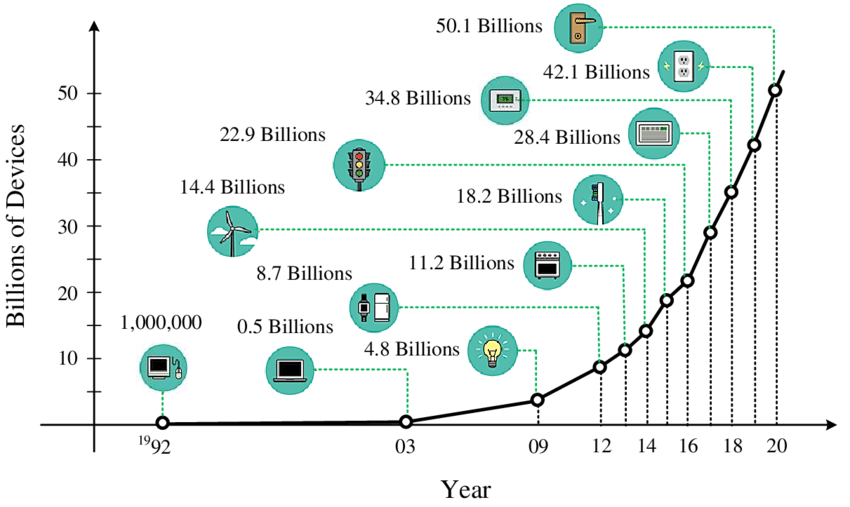
\includegraphics[scale=0.5]{graphics/chapter-1/chap1-number-of-connected-device-to-internet.png}
    \caption{Số lượng thiết bị kết nối vào mạng internet qua các năm \cite{ali2015next}}
    \label{fig:chap1-number-of-connected-device-to-internet}
\end{figure}

\begin{figure}
    \centering
    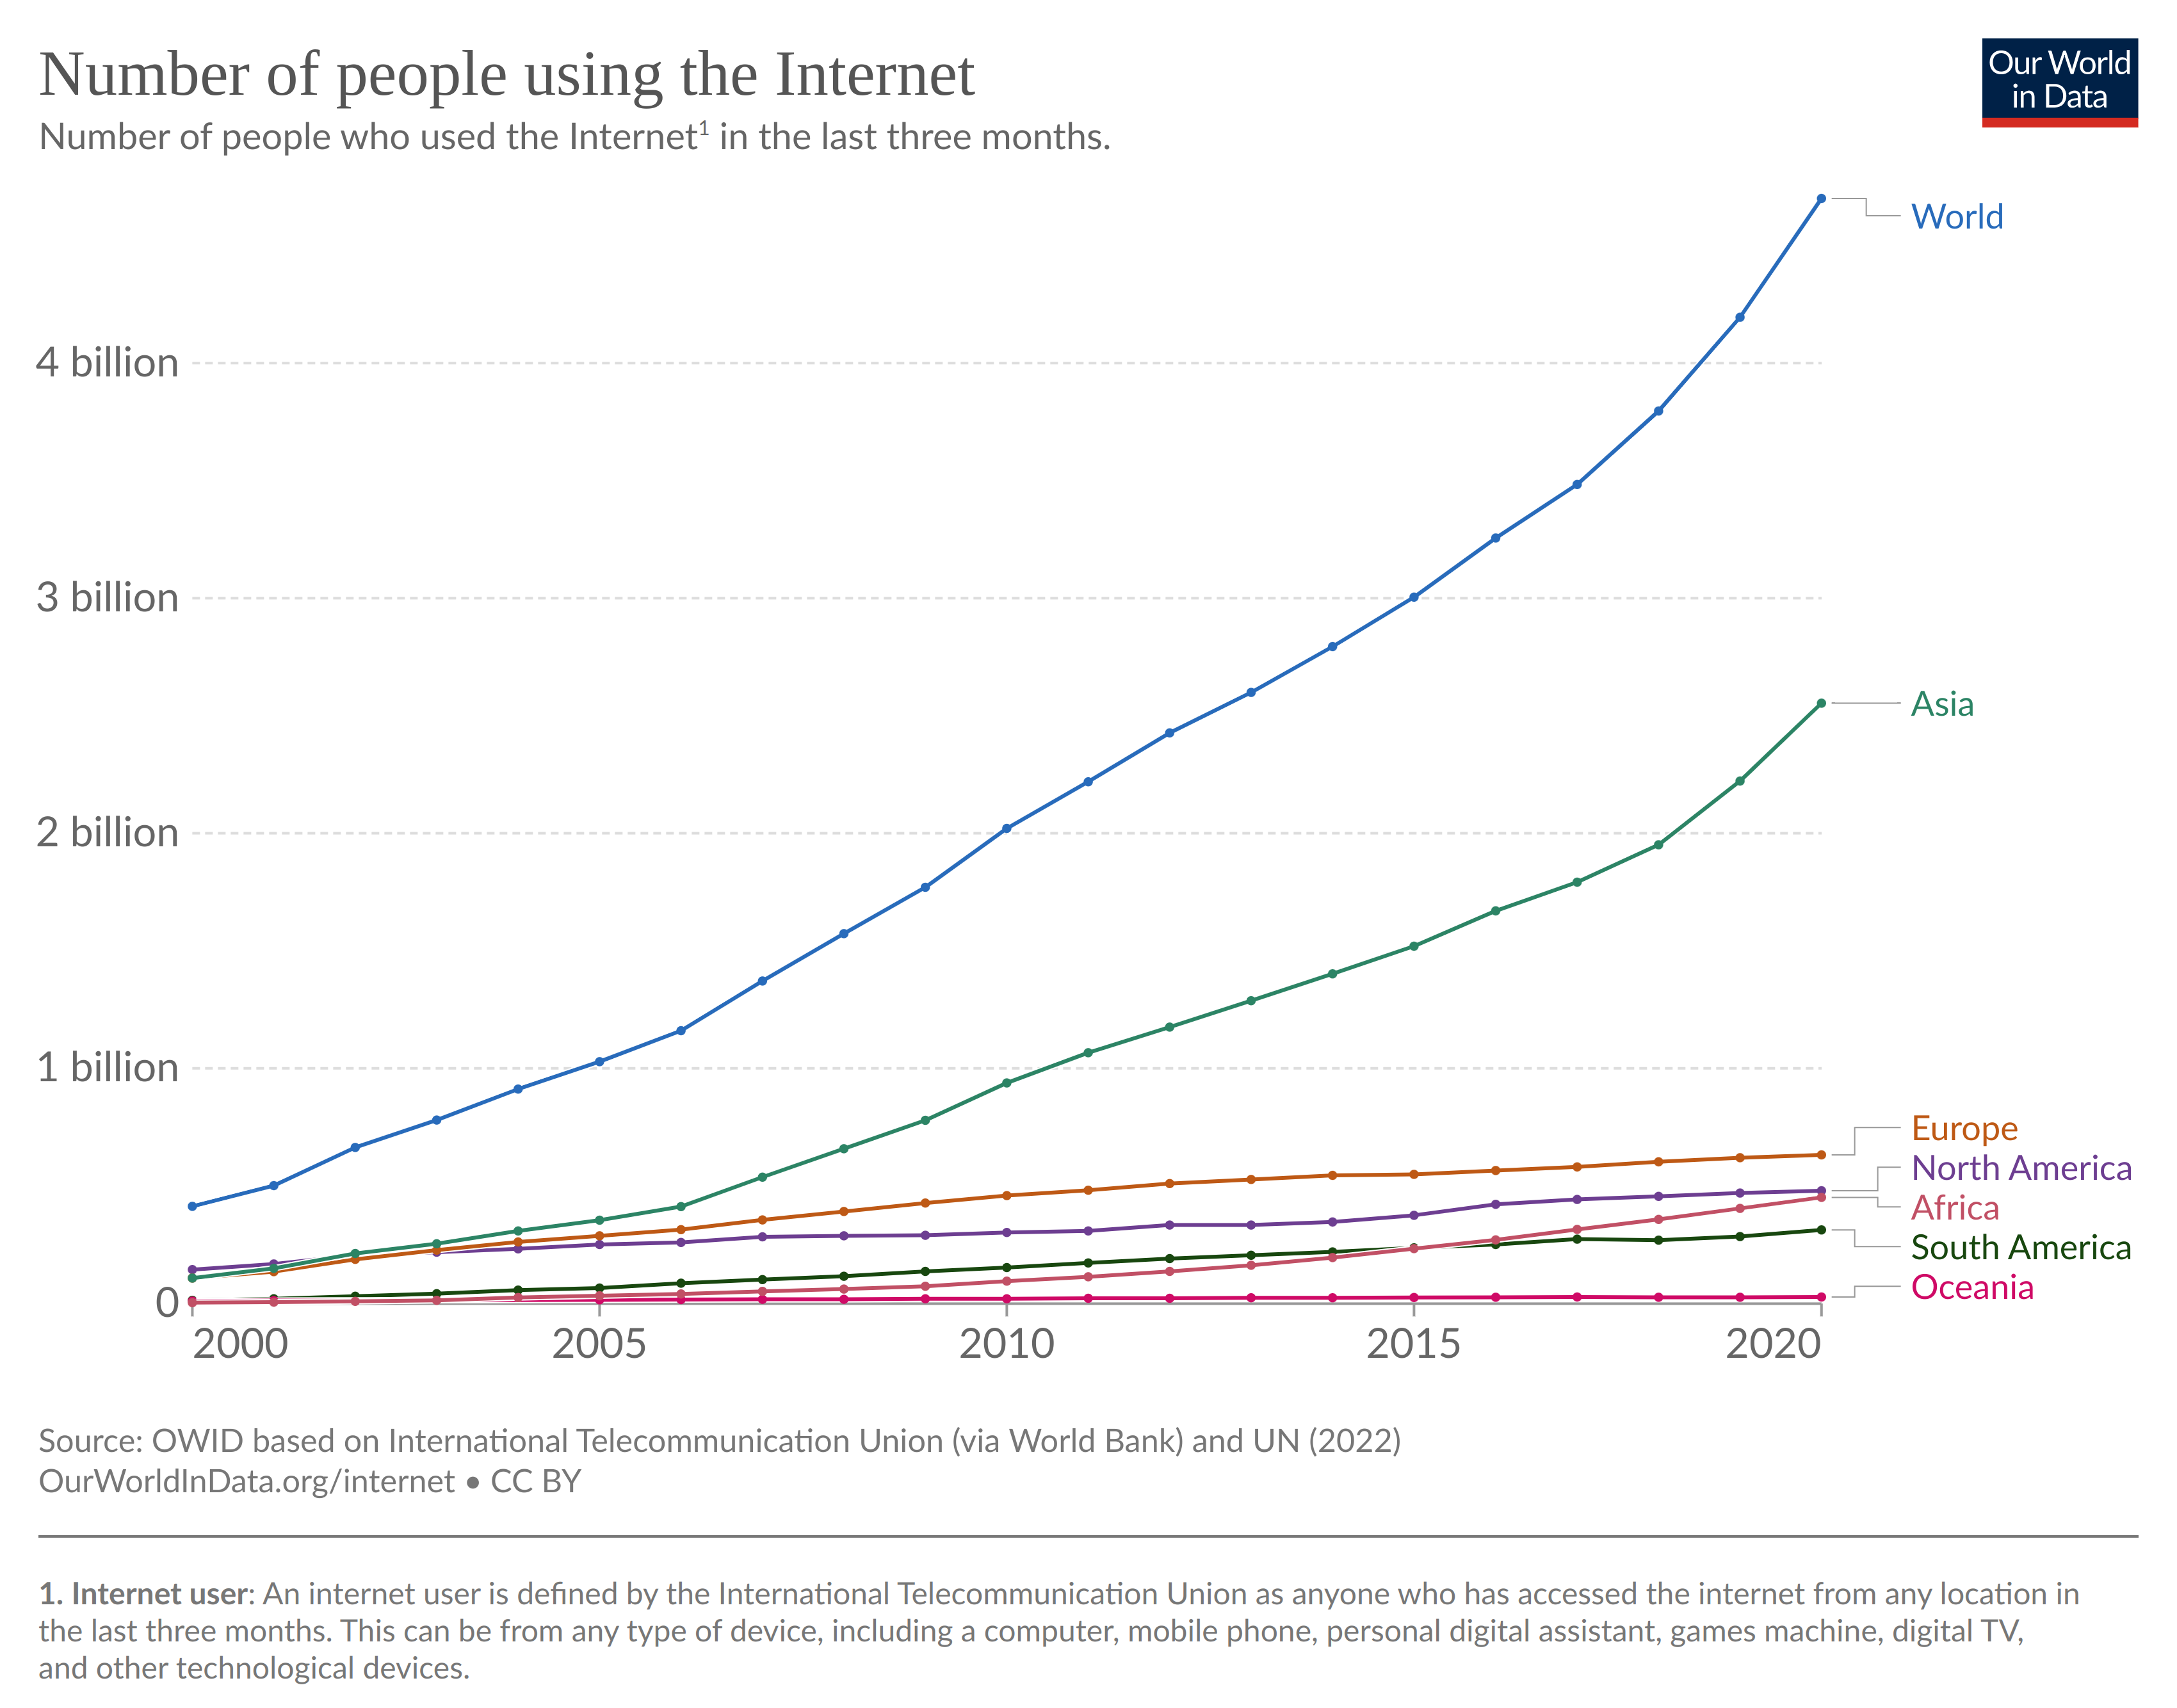
\includegraphics[scale=0.1]{graphics/chapter-1/chap1-number-of-people-use-internet.png}
    \caption{Số lượng người sử dụng internet qua các năm \cite{number2022ourworld}}
    \label{fig:chap1-number-of-people-use-internet}
\end{figure}

Ngoài những yêu cầu cấp thiết về pháp lý, phát triển các biện pháp kỹ thuật là phương thức hiệu quả, áp dụng nhanh chóng và cũng là nguồn quan trọng để có thể  tiếp tục các quy trình pháp luật sau khi bị tấn công. Kiểm thử thâm nhập (penetration testing) là một trong những phương pháp được sử dụng thường xuyên và hiệu quả để đánh giá mức độ an toàn và bảo mật của hệ thống máy tính, giảm thiểu rủi ro liên quan đến bảo mật thông tin \cite{arkin2005software}. 

Kiểm thử xâm nhập nghĩa là, thông qua vai trò như là một hacker, người làm nhiệm vụ thực hiện giả định tấn công vào ứng dụng, máy chủ thực tế, báo cáo kết quả thực hiện và đề xuất những biện pháp bảo vệ dành cho nhà phát triển. Nó có thể được thực hiện trên môi trường thử nghiệm hoặc chính môi trường thực tế. Hiện nay có nhiều công cụ được thiết kế cung cấp khả năng kiểm thử những lỗ hổng cơ bản như Nmap \cite{lyon2009nmap}, Nessus \cite{thacker2006probabilistic}, OpenVAS \cite{aksu2019first}, Metasploit Framework \cite{holik2014effective},... Tuy nhiên để có thể hiểu và phát huy các công cụ này một cách hiệu quả, vẫn cần người sử dụng đã được được đào tạo, có kỹ năng và kiến thức (trong nhiều trường hợp là kinh nghiệm) nhất định. Mặt khác, các hệ thống công nghệ thông tin ngày càng phức tạp, nhiều lớp, nhiệm vụ đánh giá bảo mật theo cách thủ công ngày càng kém hiệu quả, dần dần sẽ không còn khả thi do tỉ lệ sai sót vô ý của con người. 

Như vậy, hiển nhiên cần thiết là quá trình kiểm thử xâm nhập phải được tự động hóa. Không quá dựa nhiều vào công sức của kỹ thuật viên, nhưng cũng không bỏ hoàn toàn họ ra chỉ vì lỗi khách quan (do phải xử lý quá nhiều thông tin và thao tác).

Đây là một chủ đề không mới, nó đã được nghiên cứu nhiều năm nay. Công nghệ phát triển qua từng ngày, kỹ thuật khai thác cũng được thiết kế tinh vi hơn. Từ đó, những lỗ hổng có thể khai thác cũng tăng dần. Vấn đề đặt ra là làm thế nào một công cụ có thể học cách khai thác lỗ hổng và tích lũy kinh nghiệm này cho các lần tiếp theo. Sử dụng máy học là xu hướng hiện nay và kiểm thử  phần mềm cũng không nằm ngoài làn sóng đó. Sử dụng Reinforcement Learning (RL) có thể tận dụng kinh nghiệm thực tế từ các hành động trong quá khứ để quét và tấn công sau đó \cite{liu2020deep}. 




% \begin{figure}[!h]
%     \centering
%     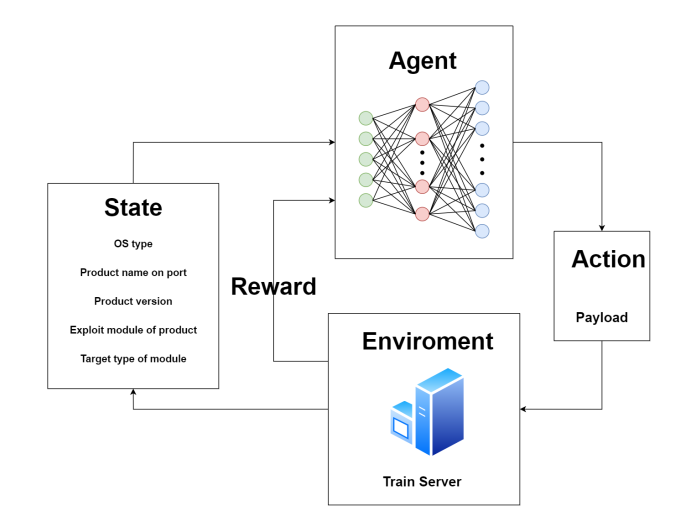
\includegraphics[scale=0.6]{graphics/chapter-1/chap1-abtractRL.png}
%     \caption{Tổng quan về học tăng cường}
%     \label{fig:chap1-abtractRL}
% \end{figure}


% Ví dụ, RL có thể được sử dụng để tạo ra các phần mềm độc hại mới có khả năng làm sai lệch các đánh giá của các công cụ kiểm như như nghiên cứu của nhóm tác giả Daniel Gibert \cite{gibert2022enhancing} hoặc nhóm tác giả Fang \cite{fang2019evading}. Từ đó cho thấy, các hệ thống thông minh dựa trên RL có tính kinh tế, mạnh mẽ, phổ biến và năng động, đặc biệt là về an ninh mạng do sự thay đổi liên tục của các vec-tơ tấn công và payload của chúng \cite{adawadkar2022cyber}. 

% Cho đến nay, đã có một số nghiên cứu liên quan đến các giải pháp tự động hóa kiểm thử thâm nhập bằng cách sử dụng học tăng cường. Trong nghiên cứu của Zhenguo và cộng sự \cite{hu2020automated}, nhóm nghiên cứu đã sử dụng học tăng cường để tìm ra đường tấn công tối ưu nhất cho mô hình mạng thực tế. Các tác giả đã sử dụng công cụ Shodan để thu thập dữ liệu máy chủ thực tế tại các địa điểm công cộng khác nhau để xây dựng các mạng mục tiêu thực tế. Sau đó kết hợp sử dụng MulVAL \cite{yousefi2018reinforcement} và Depth-First Search (DFS) để xây dựng một ma trận tấn công, cuối cùng sử dụng DQN để phân tích ma trận và tìm ra đường tấn công tối ưu nhất cho mô hình mạng. Mặc dù đạt được kết quả tốt theo đánh giá của các tác giả, việc thực hiện vẫn cần rất nhiều sự hỗ trợ từ các framework khác để có thể tự động hóa quá trình thử nghiệm thâm nhập. Trong một nghiên cứu khác, nhóm của Ryusei Maeda \cite{maeda2021automating} cũng đã tập trung vào tấn công tự động với RL sâu, nhưng nghiên cứu này tập trung vào quá trình sau khi bị tấn công. Nghiên cứu này dựa vào một mô-đun agent RL là PowerShell Empire - một mô-đun đã dừng cập nhật - nên nó không thể tiếp tục nghiên cứu và cập nhật sau này.

% Ngoài ra, tại hội nghị Arsenal 2018 Black Hat USA, Isao Takaesu đã giới thiệu DeepExploit \cite{takaesudeepexploit}, một công cụ tấn công tự động sử dụng RL để khai thác các lỗ hổng trên máy chủ. Hiện nay, các thành phần của DeepExploit yêu cầu sửa đổi thêm để hoạt động. Không có thông báo về hiệu suất thực tế của nó đối với các lỗ hổng trong thế giới thực.

% Lấy cảm hứng từ DeepExploit, trong nghiên cứu này, chúng tôi sử dụng thuật toán A3C \cite{mnih2016asynchronous} để huấn luyện agent RL. Nghiên cứu được phát triển nhằm mục đích tích lũy kinh nghiệm trong việc chọn payload chính xác, để khai thác các lỗ hổng có sẵn trong môi trường tiếp theo. Nghiên cứu tập trung vào quá trình do thám và  tấn công trên máy chủ mục tiêu thông qua Metasploit Framework, là hai giai đoạn đầu tiên của quá trình thử nghiệm thâm nhập \cite{engebretson2013basics}. Ngoài ra, sau quá trình thử nghiệm, công cụ sẽ hỗ trợ xuất các báo cáo về các lỗ hổng bị khai thác một cách trực quan, cho phép người dùng dễ dàng quan sát và đánh giá. Cuối cùng, để đánh giá hiệu suất của mô hình, công cụ kiểm tra thâm nhập tự động được áp dụng cho các kiến trúc mạng nơ-ron khác nhau trong các tình huống kế tiếp. 


\section{Mục tiêu của đề tài}

\begin{itemize}
    \item Trong đề tài này, chúng tôi xây dựng một công cụ kiểm thử xâm nhập tự động sử dụng học tăng cường sâu giúp hỗ trợ kỹ thuật viên kiểm thử phần mềm, hỗ trợ xuất báo cáo phục vụ cho nhà phát triển ứng dụng.
    \item 
    Công bố các công trình nghiên cứu khoa học phù hợp với yêu cầu đề tài.
\end{itemize}

\section{Cấu trúc báo cáo}
Nội dung báo cáo của đề tài được tổ chức như sau:
\begin{itemize}
    \item \textbf{Chương \ref{chapter1}} giới thiệu bài toán đặt ra.
    \item \textbf{Chương~\ref{chapter2}} trình bày cơ sở lý thuyết  và các nghiên cứu liên quan.
    \item \textbf{Chương~\ref{chapter3}} trình bày phương pháp và mô hình đề xuất.
    \item \textbf{Chương~\ref{chapter4}} trình bày thực nghiệm và đánh giá.
    \item \textbf{Chương~\ref{chapter5}} tổng kết đề tài và hướng phát triển.
\end{itemize}
\chapter{Cơ sở lý thuyết và các nghiên cứu liên quan}
\label{chapter2}
\section{ Kiểm thử thâm nhập}
\subsection{Tổng quan}

Như đã trình bày tại \textbf{Chương \ref{chapter1}}, dữ liệu ngày nay là tài sản, tài nguyên vô cùng quan trọng. Ngày càng nhiều những thông tin mật, tuyệt mật và riêng tư được lưu trữ trên hệ thống máy tính, nơi thông thường đều được kết nối mạng. Những thông tin này bao gồm rất nhiều lĩnh vực khác nhau như kinh tế, tài chính, y tế, giáo dục, khoa học, thậm chí là quân sự. Giá trị của những thông tin này không thể đong đếm được. Thách thức đặt ra là phải bảo vệ những thông tin này an toàn. Nếu dữ liệu được lưu trữ trong một hệ thống máy tính, bằng cách nào đó, hệ thống này phải được chứng minh rằng nó đủ an toàn và không dễ bị tấn công. Diễn tập hay thử nghiệm các bài tất công có chủ đích như là một phương pháp đắc lực, hiệu quả và có thể xác nhận.

\subsection{Phương pháp tiếp cận}

Kiểm thử xâm nhập là một cách tiếp cận để tăng cường và củng cố an ninh của hệ thống thông tin, nhưng nó chắc chắn không nói lên rằng hệ thống là hoàn toàn bất khả xâm phạm. Thông thường sẽ được thực hiện theo những kịch bản có sẵn với một danh sách các lỗi đã được công bố.

Hiện nay, có nhiều phương pháp hỗ trợ kiểm thử xâm nhập. Đây vừa là thuận lợi, vừa cũng là khó khăn khi đòi hỏi người thực hiện phải chọn phương pháp phù hợp. Người kiểm thử càng có nhiều kinh nghiệm, càng có nhiều kiến thức tốt hơn về môi trường được kiểm tra thì càng có thể đưa ra lựa chọn chính xác hơn về một phương pháp phù hợp, chẳng hạn như Open Source Security Testing Methodology Manual do ISECOM tạo và duy trì hoặc Open Web Application Security Project (OWASP) đối với các ứng dụng web và phần mềm. 

Đối với OWASP, đây là một dự án được tạo ra và duy trì bởi OWASP - một tổ chức phi lợi nhuận gồm có nhiều thành viên là các chuyên gia từ ngành phát triển ứng dụng web hoặc các chuyên gia trong lĩnh vực phần mềm. OWASP hướng tới phương pháp xây dựng những ứng dụng và dịch vụ web một cách an toàn, bằng cách mô tả những gì cần làm tại mỗi giai đoạn phát triển phần mềm để có thể đạt được mục tiêu là sự an toàn nhất có thể cho sản phẩm. Ngoài ra, OWASP cũng cung cấp một báo cáo được cập nhật thường xuyên về các nguy cơ bảo mật đối với bảo mật ứng dụng web, tập trung vào 10 rủi ro, lỗ hổng quan trọng và phổ biến nhất, được gọi là OWASP TOP 10.

OWASP đưa ra một quy trình hoặc kiến trúc của một bài kiểm tra xâm nhập phần mềm, thường chia ra làm nhiều giai đoạn. Trong đó, mỗi kết quả của giai đoạn này chính là đầu vào cho giai đoạn tiếp theo. Trong tình huống thực tế cụ thể, những giai đoạn này lại chia thành nhiều bước khác nhau để đánh giá logic của hệ thống được kiểm tra.

Các bước cụ thể có thể khác nhau, nhưng nhìn chung, chúng phải trải qua các giai đoạn sau.
\begin{itemize}
    \item Thu thập thông tin: thực hiện tìm kiếm, quét hệ thống, phần mềm, người sử dụng phần mềm, người vận hành hệ thống. Mục đích là tìm ra một lỗ hổng trong hệ thống.
    \item Dựa vào lỗ hổng đã được khám phá, tiến hành tần công thâm nhập hệ thống, mục đích là có được quyền quản trị hệ thống, tiếp tục sử dụng quyền mới để leo thang đặc quyền.
    \item Sau khi tấn công xong, xóa dấu vết của quá trình xâm nhập để không bị phát hiện cũng như truy vết.
\end{itemize}

Việc phân rã quá trình kiểm thử theo các giai đoạn khác nhau sẽ phù hợp với các loại công cụ khác nhau. Mỗi công đoạn có thể sử dụng các công cụ độc lập. Như tại bước thu thập thông tin thường sử dụng các công cụ như giám sát lưu lượng, quét cổng và phát hiện hệ điều hành để thu thập thông tin liên quan để kiểm tra lỗ hổng bảo mật trên hệ thống. Đối với giai đoạn tấn công và xâm nhập, có thể là một chương trình hoặc dữ liệu nhất định nhằm tận dụng lỗ hổng đã được phát hiện và giành được quyền truy cập hệ thống. Mặc dù các môi trường được kiểm tra có những khác nhau, hầu hết các bước thường giống nhau và được thực hiện đầy đủ. Nhiều công cụ đã được phát triển để hỗ trợ cho chính xác một công đoạn trong quá trình kiểm thử.

\section{Học tăng cường}
\subsection{Tổng quan}



Học tăng cường là một nhánh trong học máy. \textbf{Hình \ref{fig:chap2-rl-overview}} mô tả mô hình học tăng cường cơ bản. Một agent $B$ nhận đầu vào là tín hiệu $i$ từ môi trường, trạng thái $s$ của môi trường, chọn một hành động $a$ để thực hiện. Hành động này làm thay đổi trạng thái của môi trường và gửi chúng tới agent thông qua một tín hiệu \textit{vô hướng} $r$. $B$ được thiết kế để chọn các hành động có xu hướng làm tăng tổng giá trị của môi trường. Nó được thiết kế để làm điều này bằng cách thử và sai một cách có hệ thống \cite{kaelbling1996reinforcement}. 


Học giám sát cũng là một nhánh lớn được nghiên cứu. Dữ liệu huấn luyện của nó là một cặp gồm đối tượng đầu vào và đối tượng đầu ra mong muốn. Đầu ra của hàm huấn luyện có thể là một giá trị liên tục hoặc một nhãn của đầu vào. Nhiệm vụ của hàm học giám sát là dự đoán giá trị đầu ra cho bất kỳ đầu vào hợp lệ, dựa trên tập dữ liệu đã được huấn luyện. Để làm được điều này, hàm học giám sát phải tổng quát hóa dữ liệu huấn luyện, dựa trên đó để đoán được đầu ra của những tình huống chưa gặp phải \textit{một cách hợp lý}.


\begin{figure}
    \centering
    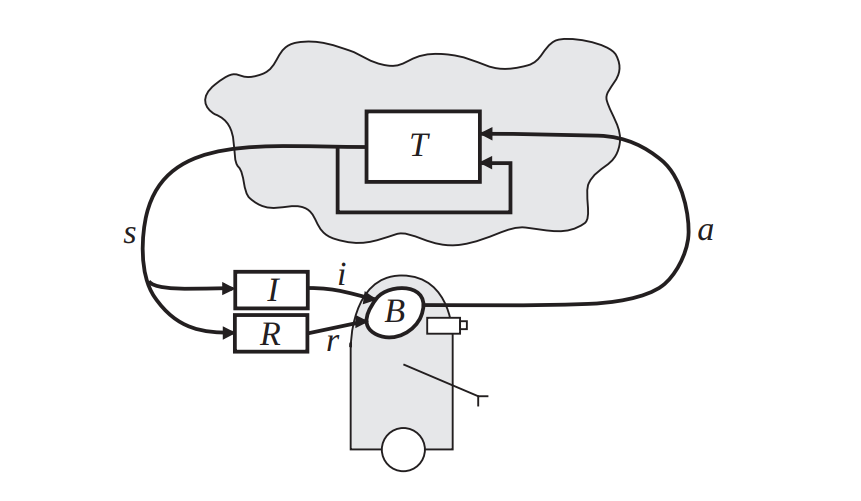
\includegraphics[scale=0.5]{graphics/chapter-2/chap2-rl-overview.png}
    \caption{Tổng quan về học tăng cường}
    \label{fig:chap2-rl-overview}
\end{figure}


Ở một khía cạnh khác, chúng ta có một kỹ thuật khác gọi là học không giám sát. Học không giám sát không có bất kỳ nhãn nào được gán cho dữ liệu, mục tiêu là tìm hiểu một số cấu trúc ẩn của tập dữ liệu hiện có, điển hình là bài toán phân cụm dữ liệu. Học không giám sát khác với học có giám sát ở chỗ đầu ra đúng tương ứng cho mỗi đầu vào là không biết trước. Chúng ta sẽ xem các đối tượng đầu vào như một tập các biến ngẫu nhiên, sau đó tìm cách xây dựng một mô hình mật độ kết hợp cho tập dữ liệu đó. Một phương pháp học tập không giám sát khác đang ngày càng trở nên phổ biến là mạng sinh đối kháng (GANs).

\begin{figure}
    \centering
    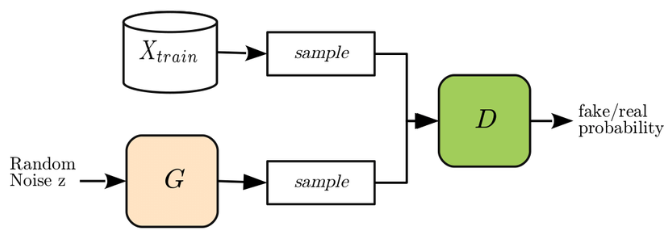
\includegraphics[scale=0.6]{graphics/chapter-2/chap2-gan-overview.png}
    \caption{Tổng quan về học không giám sát sử dụng mạng sinh đối kháng}
    \label{fig:chap2-gan-overview}
\end{figure}


Học tăng cường được nghiên cứu trong đề tài là một phương pháp ở giữa học giám sát và học không giám sát. Nó sử dụng nhiều phương pháp học giám sát đã được thiết kế tốt như mạng nơ-ron sâu dể biểu diễn dữ liệu hoặc làm nền tảng trước khi học tăng cường. Nó có thể tận dụng kinh nghiệm thực tế từ các mô hình đã được huấn luyện bằng học giám sát để quét và tấn công sau đó \cite{liu2020deep}.

% \begin{figure}[!h]
%     \centering
%     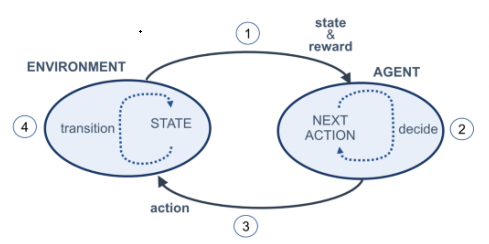
\includegraphics[width=0.9\textwidth]{graphics/chapter-2/chap2-RL_overview.PNG}
%     \caption{Tổng quan về học tăng cường.} 
%     \label{fig:chap2-RL_overview}
% \end{figure}

\subsection{Các thành phần chính}
Mọi lĩnh vực khoa học và kỹ thuật đều có những giả định và hạn chế riêng. Chúng tôi không muốn nói việc học có giám sát là tốt hay không tốt, tuy nhiên có những vấn đề mà học giám sát không thể giải quyết hiệu quả, thay vào đó là học tăng cường. 

Trong học tăng cường, không có các cặp dữ liệu đầu vào và đầu ra đúng, các hành động tối ưu cũng không được đánh giá đúng sai một cách tường mình, thay vào đó là hệ thống phần thưởng nhất định. Hoạt động trực tiếp của tác nhân là thứ được quan tâm. Các vấn đề của học tăng cường liên quan đến việc học những gì cần làm thông qua việc ánh xạ tình huống thành hành động để tối đa hóa phần thưởng bằng số, trong đó có việc tìm kiếm sự cân bằng giữa khám phá (những kiến thức mới chưa được học) và khai thác (những kiến thức đã được học). Nhìn chung, học tăng cường bao gồm 2 thực thể chính là Tác nhân và Môi trường, tương tác với nhau thông qua các kênh giao tiếp của chúng là Hành động, Phần thưởng và Quan sát.


\section{Các nghiên cứu liên quan}

RL không phải là một lĩnh vực mới xuất hiện gần đây, nó đã được nghiên cứu nhiều năm. Các giải pháp có triển vọng trong RL . Ví dụ, RL có thể được sử dụng để tạo ra các phần mềm độc hại mới có khả năng làm sai lệch các đánh giá của các công cụ kiểm như như nghiên cứu của nhóm tác giả Daniel Gibert \cite{gibert2022enhancing} hoặc nhóm tác giả Fang \cite{fang2019evading}. Từ đó cho thấy, các hệ thống thông minh dựa trên RL có tính kinh tế, mạnh mẽ, phổ biến và năng động, đặc biệt là về an ninh mạng do sự thay đổi liên tục của các vec-tơ tấn công và payload của chúng \cite{adawadkar2022cyber}. 


Cho đến nay, đã có một số nghiên cứu liên quan đến các giải pháp tự động hóa kiểm thử thâm nhập bằng cách sử dụng học tăng cường. Trong nghiên cứu của Zhenguo và cộng sự \cite{hu2020automated}, nhóm nghiên cứu đã sử dụng học tăng cường để tìm ra đường tấn công tối ưu nhất cho mô hình mạng thực tế. Các tác giả đã sử dụng công cụ Shodan để thu thập dữ liệu máy chủ thực tế tại các địa điểm công cộng khác nhau để xây dựng các mạng mục tiêu thực tế. Sau đó kết hợp sử dụng MulVAL \cite{yousefi2018reinforcement} và Depth-First Search (DFS) để xây dựng một ma trận tấn công, cuối cùng sử dụng DQN để phân tích ma trận và tìm ra đường tấn công tối ưu nhất cho mô hình mạng. Mặc dù đạt được kết quả tốt theo đánh giá của các tác giả, việc thực hiện vẫn cần rất nhiều sự hỗ trợ từ các framework khác để có thể tự động hóa quá trình thử nghiệm thâm nhập. Trong một nghiên cứu khác, nhóm của Ryusei Maeda \cite{maeda2021automating} cũng đã tập trung vào tấn công tự động với RL sâu, nhưng nghiên cứu này tập trung vào quá trình sau khi bị tấn công. Nghiên cứu này dựa vào một mô-đun agent RL là PowerShell Empire - một mô-đun đã dừng cập nhật - nên nó không thể tiếp tục nghiên cứu và cập nhật sau này.

Ngoài ra, tại hội nghị Arsenal 2018 Black Hat USA, Isao Takaesu đã giới thiệu DeepExploit \cite{takaesudeepexploit}, một công cụ tấn công tự động sử dụng RL để khai thác các lỗ hổng trên máy chủ. Hiện nay, các thành phần của DeepExploit yêu cầu sửa đổi thêm để hoạt động. Không có thông báo về hiệu suất thực tế của nó đối với các lỗ hổng trong thế giới thực.

Lấy cảm hứng từ DeepExploit, trong nghiên cứu này, chúng tôi sử dụng thuật toán A3C \cite{mnih2016asynchronous} để huấn luyện agent RL. Nghiên cứu được phát triển nhằm mục đích tích lũy kinh nghiệm trong việc chọn payload chính xác, để khai thác các lỗ hổng có sẵn trong môi trường tiếp theo. Nghiên cứu tập trung vào quá trình do thám và  tấn công trên máy chủ mục tiêu thông qua Metasploit Framework, là hai giai đoạn đầu tiên của quá trình thử nghiệm thâm nhập \cite{engebretson2013basics}. Ngoài ra, sau quá trình thử nghiệm, công cụ sẽ hỗ trợ xuất các báo cáo về các lỗ hổng bị khai thác một cách trực quan, cho phép người dùng dễ dàng quan sát và đánh giá. Cuối cùng, để đánh giá hiệu suất của mô hình, công cụ kiểm tra thâm nhập tự động được áp dụng cho các kiến trúc mạng nơ-ron khác nhau trong các tình huống kế tiếp. 

\chapter{Phương pháp và mô hình đề xuất }
\label{chapter3}
\section{Tổng quan hệ thống}


Kế thừa những điểm tốt trong kiến trúc của DeepExploit \cite{takaesudeepexploit}, tổng quan mô hình đề xuất học tăng cường sâu gồm:

\begin{itemize}
    \item Một server làm nhiệm vụ train cho agent
    \item State của môi trường bao gồm 5 thuộc tính: OS type, product name on port, product version, exploit module of product, target type of module
    \item Một action chính là payload thực hiện lên trên môi trường đặt tại server train
    \item Một hàm reward có nhiệm vụ "cho điểm" nếu action được đánh giá tốt.
\end{itemize}
được thể hiện trong \textbf{Hình \ref{fig:chap3-rlauto-pentest}}. Học tăng cường sâu là sự kết hợp của học tăng cường và học sâu. Trong thực tế, phần "sâu" ở đây là về việc sử dụng mạng nơ-ron với các tham số trọng số $\theta$ để xấp xỉ hàm giá trị $Q(s, a)$ trong quá trình đào tạo agent RL.

\begin{figure}[!h]
    \centering
    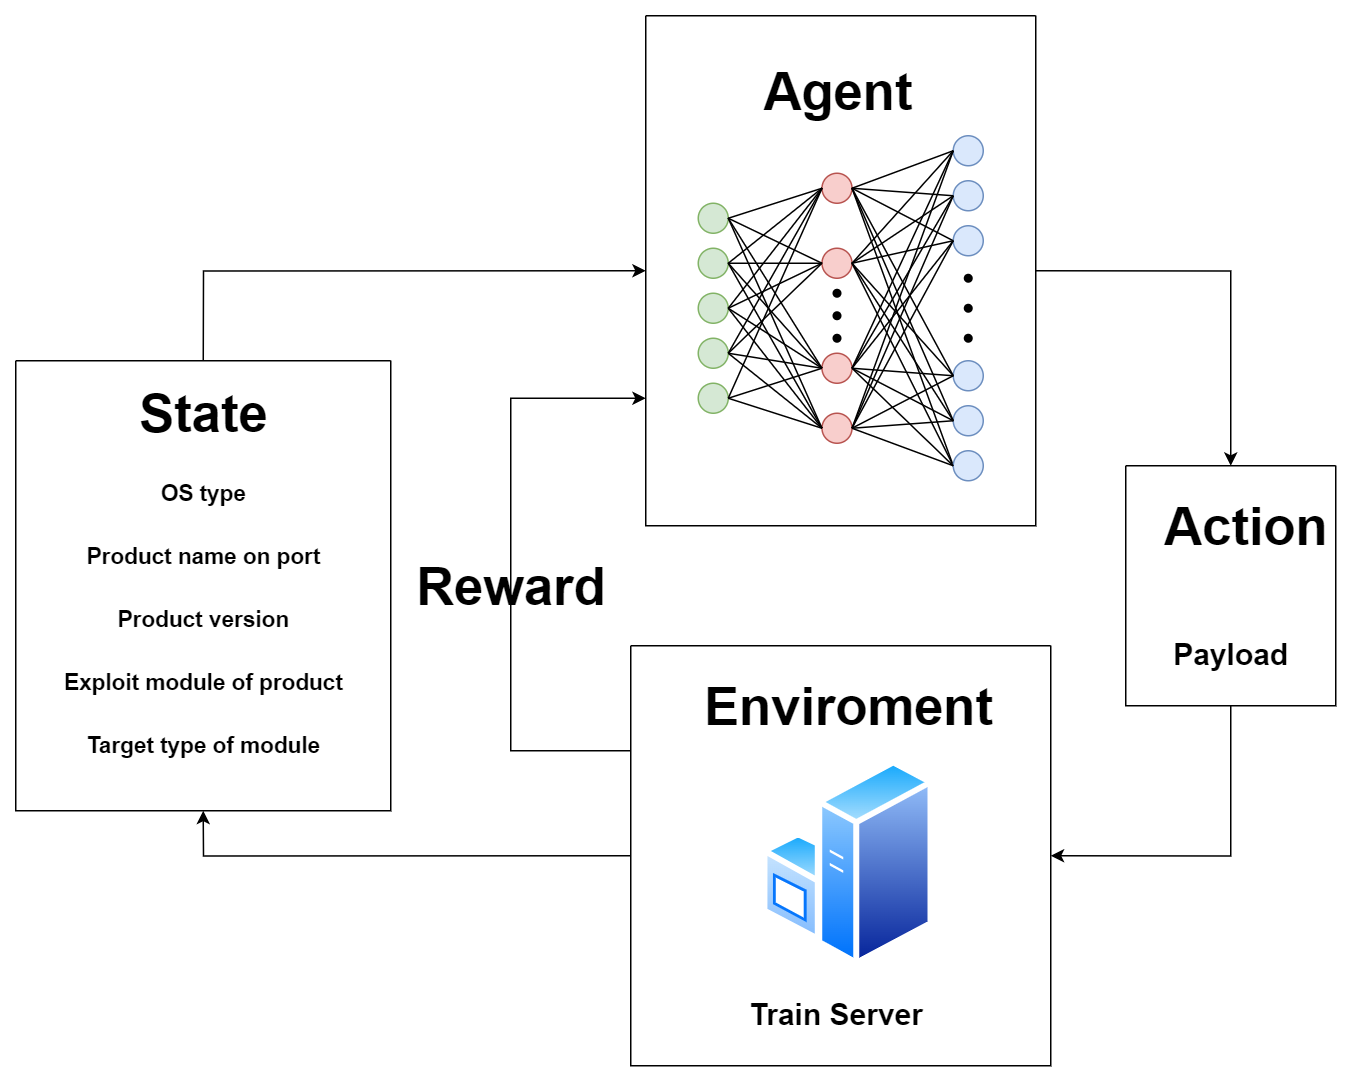
\includegraphics[scale=0.3]{graphics/chapter-3/chap3-rlauto-pentest.png}
    \caption{Kiến trúc tổng thể }
    \label{fig:chap3-rlauto-pentest}
\end{figure}


\section{Mô hình Quyết định Markov (MDP)}

Một vấn đề đặt ra là quá trình học tăng cường tác động liên tục qua lại với môi trường huấn luyện nó. Để chỉ định các ràng buộc (mà biến thiên qua quá trình huấn luyện) giữa môi trường với agent, mỗi vòng lặp huấn luyện sử dụng mô hình quyết định Markov (MDP) \cite{levin1998using}.

MDP là một khung lý thuyết thường được sử dụng để mô tả các tình huống quyết định trong môi trường chưa xác định và biểu diễn quá trình ra quyết định trong điều kiện không hoàn hảo. Nó gồm các thành phần chính như trạng thái của môi trường, không gian vector hoạt động và hàm reward. Trạng thái là những nhiều diễn tình trạng môi trường hiện tại, hành động là những lựa chọn mà agent có thể thực hiện để thay đổi trạng thái, trong khi hàm reward thực hiện đánh giá hiệu quả của hành động đó.

Một điểm quan trọng trong MDP là tính chất Markov, có nghĩa là trạng thái tiếp theo chỉ phụ thuộc vào trạng thái hiện tại và hành động được thực hiện, không phụ thuộc vào quá khứ. Điều này giúp giảm đáng kể kích thước của không gian trạng thái, làm cho quyết định trở nên hiệu quả hơn.

\begin{itemize}
    \item \textbf{Trạng thái} $s$ bao gồm 5 thuộc tính như sau:
    
        \begin{itemize}
            \item OS type
            \item Product name on port
            \item Product version
            \item Exploit module of product
            \item Target type of module on Metasploit framework
        \end{itemize}

    Dựa trên trạng thái $s$, agent RL thực hiện 1 hành động $a$ để khai thác các lỗ hổng. Và \textbf{hành động} $a =$ \{Excellent, Great, Good\}  là một vector của 3 loại đánh giá trong Metasploit.
    \item \textbf{Phần thưởng} $r$ được xác định là tích cực nếu payload được chọn thành công và tiêu cực nếu payload được chọn thất bại. Agent được huấn luyện để tối đa hóa kỳ vọng của phần thưởng tích lũy có chiết khấu dựa trên công thức \textbf{(\ref{reward})}.
    \begin{equation}
        R = \sum^{T}_{t=1} \gamma^{t-1} r_t  
        \label{reward}
    \end{equation}
    với $\gamma \in (0, 1]$  hệ số chiết khấu tương lai.
    \item \textbf{Chính sách} $\pi$ là một hàm để quyết định hành động $a$ có sẵn cho trạng thái $s$.
    \item \textbf{Hàm giá trị} $V_{\pi}(s)$ ước tính mức độ tốt của việc thực hiện một hành động $a$ cụ thể theo chính sách $\pi$ trong trạng thái $s$.
    \begin{equation}
        V_{\pi}(s) = E\{\sum^{\infty}_{t=0} \gamma^{t} r_t  \}
        \label{vvalue}
    \end{equation}
    \item \textbf{Hàm giá trị hành động tối ưu} $Q^*(s_t, a)$ được thể hiện trong Công thức \textbf{(\ref{qvalue})} ước tính phần thưởng kỳ vọng của việc thực hiện một hành động $a$ tại $t^{th}$ trạng thái $s_t$. 
    \begin{equation}
        Q^*(s_t, a) = E\{r_{t} + \gamma \max_{a'} Q^*(s_{t+1},a')\}
        \label{qvalue}
    \end{equation}
\end{itemize}

\section{Huấn luyện tác nhân Học tăng cường sâu}

\subsection{Thuật toán Asynchronous Advantage Actor Critic - A3C}

Bản chất của học tăng cường (RL) dựa trên nguyên tắc phần thưởng, tức là thử - sai và điều chỉnh. Trong số nhiều mô hình RL, A3C là một policy gradient algorithm có chính sách $\pi(s_t,a;\theta)$ và hàm ước tính giá trị $V(s_t;\theta)$. Ý nghĩa của 3 chữ cái A trong thuật toán A3C \cite{mnih2016asynchronous} được mô tả như sau:

\begin{itemize}
    \item \textbf{Advantage:} một đặc điểm nơi thay vì sử dụng giá trị phần thưởng có chiết khấu $\gamma$ để cho agent biết hành động nào tốt trong tương lai, chúng ta sử dụng giá trị của hàm \textit{"advantage"}. Điều này agent RL học các phần thưởng tốt hơn. Giá trị \textit{advantage} được cho bởi biểu thức: $A = Q(s,a) - V(s)$
    \item \textbf{Actor-Critic:} một đặc điểm là A3C kết hợp dự đoán hàm giá trị $V$ cũng như chính sách tối ưu $\pi(s)$ (tức là phân phối xác suất của không gian hành động). Agent học sử dụng giá trị của hàm giá trị (Critic) để cập nhật hàm chính sách (Actor). 
    \item \textbf{Asynchronous:} A3C sử dụng nhiều agent, mỗi agent có các tham số mạng nơ-ron riêng và một bản sao của môi trường. Những agent này tương tác với môi trường của chúng một cách không đồng bộ, học với mỗi tương tác. Mỗi khi chúng tích lũy được "kinh nghiệm", nó sẽ đóng góp "kiến thức" vào \textit{Mạng toàn cục}, cũng chính là mạng quản lý chúng. Như vậy, thay vì chỉ học bằng một agent, các agent học song song và tựu trung, mô hình sẽ được huấn luyện nhanh hơn.
\end{itemize}

Cấu trúc của mô hình A3C với 2 agent học song song thể hiện trong \textbf{Hình \ref{fig:chap3-a3cParallel}}.

\begin{figure}[!h]
    \centering
    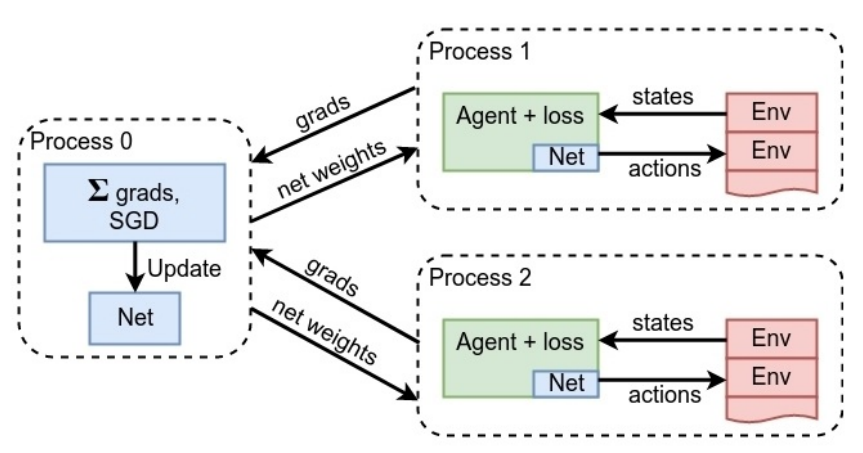
\includegraphics[scale=0.8]{graphics/chapter-3/chap3-a3cParallel.PNG}
    \caption{Mô hình A3C với hai agent học song song}
    \label{fig:chap3-a3cParallel}
\end{figure}


\subsection{Huấn luyện  agent với thuật toán A3C}

\begin{figure}[!h]
    \centering
    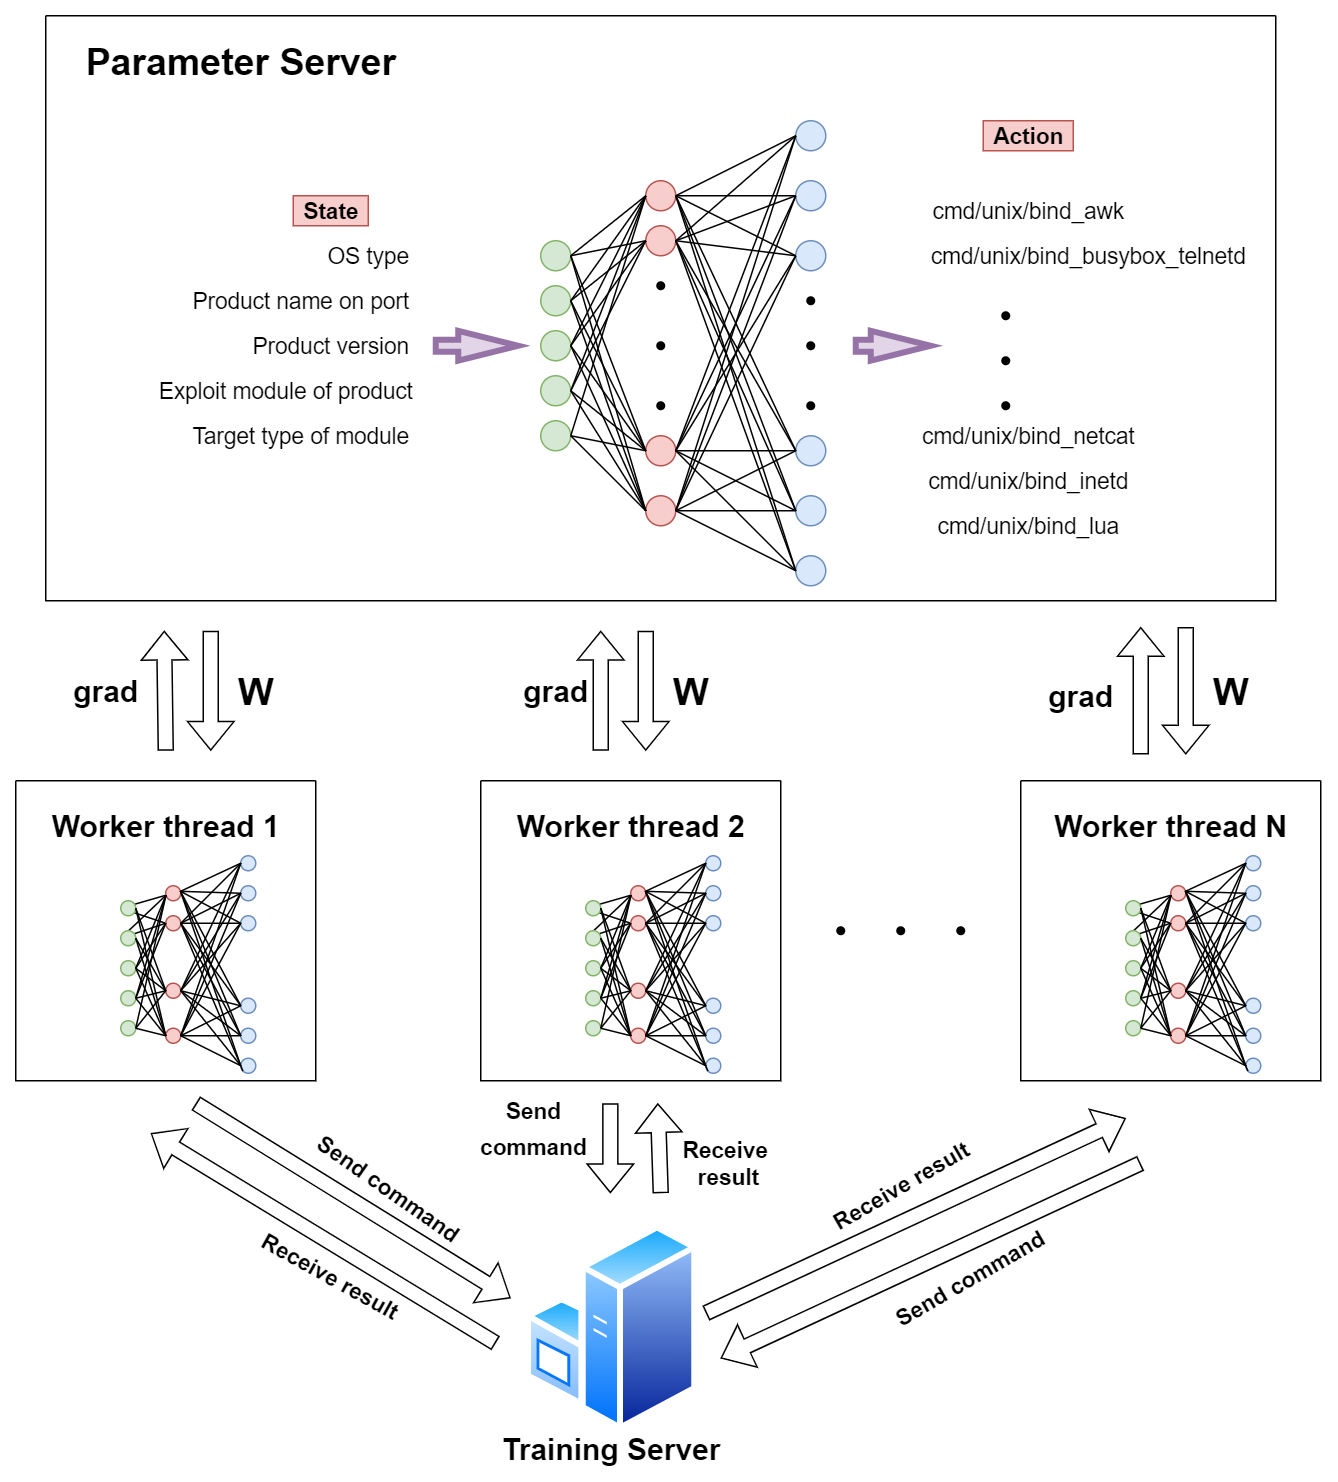
\includegraphics[scale=0.3]{graphics/chapter-3/chap3-RLA3C_AutoPentest.png}
    \caption{Chiến lược học tăng cường sâu với nhiều agent} 
    \label{fig:chap3-RLA3C_AutoPentest}
\end{figure}

Giả sử chúng ta định nghĩa hàm $J(\pi)$ như trong công thức \textbf{(\ref{eq5})}, là một phần thưởng có chiết khấu cho sự khớp trung bình $\pi$ qua tất cả các agent, bắt đầu với trạng thái đầu tiên $s_0$.
\begin{equation}
J(\pi) = E_p(s_0)[V(s_0)]
\label{eq5}
\end{equation}

Để cải thiện con số này, chúng ta cần tính toán độ dốc của $J_{\pi}$ với hàm ưu điểm \textit{A(s,a)}, như trong công thức \textbf{(\ref{eq6})}:
\begin{equation}
\bigtriangledown_{(\theta)}J_{\pi} = E_{s\sim_{\pi},a\sim\pi_{s}} [ A(s,a).\bigtriangledown_{(\theta)} Log \pi(a||s) ]
\label{eq6}
\end{equation}

Trong đó, hàm ưu điểm \textbf{A(s,a)} cho biết lợi ích của việc thực hiện hành động \textit{a} trong trạng thái \textit{s}. $\bigtriangledown_{(\theta)} Log \pi(a||s)$ cho biết một hướng mà xác suất thành công của hành động tăng lên. Cả hai trong những điều này nằm trong kỳ vọng của phân phối trạng thái và hành động của $\pi$. Tuy nhiên, chúng ta không thể tính toán chính xác nó trên mọi trạng thái và mọi hành động. Thay vào đó, chúng ta có thể sử dụng tính chất trung bình của các mẫu với phân phối xác suất. Do đó, chúng ta chỉ cần để agent chạy trong môi trường và ghi lại các mẫu \textit{(s,a,r,s')}. Sau đó, chúng ta sử dụng công thức trên để tìm một xấp xỉ của độ dốc $\bigtriangledown_{(\theta)}J_{\pi}$ và cập nhật chính sách một lần nữa.

Điểm cốt lõi của học tăng cường là thực hiện các hành động chính xác tại các trạng thái đầu vào khác nhau thông qua việc thử - sai dựa trên kết quả của các kinh nghiệm trước đó. Kết quả là, khả năng tự động exploit sẽ chính xác và ít tốn thời gian hơn. Ngoài ra, mỗi luồng công việc hoạt động như một agent Hhọc song song với [PS] - Máy chủ Tham số và [WT] - Luồng Công việc, như được miêu tả trong Hình \textbf{\ref{fig:chap3-RLA3C_AutoPentest}}. Cơ chế học tập của mô hình đã nêu trên được mô tả như sau:

\begin{itemize}
    \item \textbf{Bước 1:} [PS] khởi tạo trọng số mạng (w) với các giá trị ngẫu nhiên.
    \item \textbf{Bước 2:} [PS] sao chép trọng số mạng (w) cho các luồng công việc.
    \item \textbf{Bước 3:} [WT]  nhập trạng thái hiện tại vào mạng và chọn một số hành động.
    \item \textbf{Bước 4:} [WT] nhận phần thưởng cho các hành động. 

Vì trạng thái thay đổi khi một hành động được thực hiện, điều này được gọi là \textbf{"trạng thái tiếp theo"}. 
    \item \textbf{Bước 5:} [WT] lưu một bộ tứ gồm trạng thái hiện tại, hành động, phần thưởng và trạng thái tiếp theo như kinh nghiệm trong bộ nhớ.

    \item \textbf{Bước 6:} [WT] lặp lại các bước 3 đến 5 ở trên.
    \item \textbf{Bước 7:} [WT] sau khi tích lũy một lượng kinh nghiệm nhất định, tính gradient của mạng (grad) bằng cách sử dụng các kinh nghiệm trong bộ nhớ (trạng thái hiện tại, hành động, phần thưởng, trạng thái tiếp theo).
    \item \textbf{Bước 8:} [WT] đẩy grad lên máy chủ tham số. 
    \item \textbf{Bước 9:} [PS] cập nhật trọng số mạng (w) bằng cách sử dụng grad được đẩy từ mỗi luồng công việc. 

    \item \textbf{Bước 10:} Quay lại Bước 2 ở trên.
\end{itemize}

Theo cách này, nhiều tác nhân làm việc không đồng bộ trên các nhiệm vụ và chia sẻ kinh nghiệm của chúng để tăng tốc quá trình học.
\chapter{Thực nghiệm và đánh giá}
\label{chapter4}
\section{Triển khai}
%chi tiet ve cach lap trinh, cai dat
Công cụ được triển khai bằng Python cho thiết lập luồng A3C và TensorFlow và Keras cho việc triển khai học máy. Để thu thập thông tin về mục tiêu, chúng tôi sử dụng API RPC của Metasploit và Nmap thông qua msfconsole. Kết quả quét được trả về và lưu trong một tệp .xml.

Sau khi thu thập thông tin để xác định hệ thống mục tiêu, agent RL tool lấy danh sách các mô-đun và payload từ Metasploit để exploit qua RPC API. Kết quả exploit được lưu trong tệp .csv để sử dụng cho lần exploit tiếp theo. Các mô-đun trong Metasploit mà agent RL chọn có loại xếp hạng là: xuất sắc, tuyệt vời, tốt. Tiếp theo, agent RL tạo ra danh sách các mô-đun, payload và target với từng dịch vụ đã được liệt kê trong file .xml. Sau đó, các loại thông tin này được sử dụng để huấn luyện RL agent để học cách tự động exploit các dịch vụ đó trong tương lai.

Mạng neural sâu để huấn luyện RL agent được thiết kế với các thiết lập sau: 
\begin{itemize}
    \item Input layer: Lớp này có 5 đơn vị, đại diện cho 5 thuộc tính trạng thái.
    \item Hidden layers: Số lượng lớp ẩn và các đơn vị tương ứng được tùy chỉnh cho các kịch bản thí nghiệm.
    \item Output layer: Nó bao gồm 556 đơn vị, đại diện cho 556 tải trọng khác nhau để khai thác.
\end{itemize}

Trong đó, hàm kích hoạt giữa các lớp ẩn và lớp đầu vào là \textit{relu}. Bên cạnh đó, hàm \textit{softmax} được sử dụng để chỉ ra payload nào trong tập output nên được chọn, tương ứng với mỗi môi trường của target.

Các thông số để huấn luyện agent RL được thể hiện trong \textbf{Bảng \ref{tab:a3c_parameter}}.

\begin{table}[!h]
    \centering
    \caption{Các tham số cho thuật toán học tăng cường}
    \label{tab:a3c_parameter}
    \begin{tabular}{|c|c|}
    \hline
    \textbf{Parameter}      & \textbf{Value} \\ 
    \hline
    Gamma                   & 0.99  \\ 
    \hline
    Epsilon greedy start    & 0.5   \\ 
    \hline
    Epsilon greedy stop     & 0     \\ 
    \hline
    RMSprop learning rate   & 0.005 \\ 
    \hline
    RMSProp decay           & 0.99  \\ 
    \hline
    Loss coefficient        & 0.5   \\ 
    \hline
    Loss entropy   coefficient & 0.01  \\ 
    \hline
    Number of test   worker    & 1     \\ 
    \hline
    Greedy rate                & 0.8   \\ 
    \hline
    \end{tabular}
\end{table}



\section{Môi trường thí nghiệm}

Như các máy chủ huấn luyện, chúng tôi sử dụng 5 máy ảo (VM) Metasploitable2. Ngoài ra, chúng tôi cài đặt 5 VM chạy hệ điều hành Kali Linux, như được hiển thị trong Bảng \textbf{\ref{tab:VM_TB}}. Công cụ dựa trên RL sau đó được cài đặt trên mỗi VM. Nó cũng thay đổi các tham số DRL tương ứng với các kịch bản thử nghiệm, được liệt kê trong Bảng \textbf{\ref{tab:NN_TB}} và Bảng \textbf{\ref{tab:Thread_Trial}}. \\

\begin{table}[!h]
    \centering
    \caption{Cấu hình máy ảo}
    \label{tab:VM_TB}
    \begin{tabular}{|c|c|c|c|} \hline
        \textbf{Name of VMs} &\textbf{Operating System} &\textbf{RAM} &\textbf{CPU} \\ 
        \hline
         Penetration Testing &Kali Linux &12 GB &4 cores \\ 
         \hline
        Testing Server &Ubuntu 18.04 &12 GB &4 cores \\ 
        \hline
    \end{tabular}
    
\end{table}


\begin{table}[!h]
    \centering
    \caption{Danh sách các dịch vụ chứa lỗ hổng trong môi trường thử nghiệm.}
    \label{tab:ServiceTB}
    \begin{tabular}{|c|c|c|c|}
    \hline
    \textbf{Service}     & \textbf{Port}  & \textbf{Operating System}  & \textbf{CVE}  \\ 
    \hline
    Samba       & 445   & Docker Ubuntu  & CVE-2017-7494      \\ 
    \hline
    WebLogic    & 7001  & Docker Ubuntu  & CVE-2017-10271      \\ 
    \hline
    PostgreSQL  & 5432  & Docker Ubuntu  & CVE-2019-9193     \\ 
    \hline
    Supervisor  & 9001  & Docker Ubuntu  & CVE-2017-11610    \\ 
    \hline
    \end{tabular}
\end{table}

Bên cạnh đó, như một máy chủ thử nghiệm, chúng tôi sử dụng 5 máy ảo chạy hệ điều hành Ubuntu 18.04 với cấu hình được hiển thị trong Bảng \textbf{\ref{tab:VM_TB}}. Tất cả các dịch vụ có lỗ hổng được liệt kê trong Bảng \textbf{\ref{tab:ServiceTB}} tồn tại trên mỗi máy ảo.

\section{Kịch bản thí nghiệm}

Để đánh giá hiệu quả của kiểm thử tự động dựa trên RL agent, nhóm nghiên cứu và thí nghiệm để so sánh với phương pháp kiểm thử ngẫu nhiên. Các chỉ số đánh giá bao gòm:

\begin{itemize}
    \item Tỷ lệ thành công của các cuộc khai thác (Total training time).
    \item Tỷ lệ thành công của các cuộc khai thác (The success rate of exploits).
    \item Số bước mà RL agent phải thực hiện để chọn payload khai thác thành công (The number of steps the RL agent must take to select a successful exploit payload).
\end{itemize}

Trong đề tài này, lớp đầu vào đại diện cho số lượng thuộc tính trạng thái, trong khi lớp đầu ra tương ứng với hành động được thực hiện bởi RL agent. Do đó, chúng đều có kích thước cố định. Việc đánh giá sẽ dựa vào thay đổi số lượng lớp của mạng neural. Mặc dù các lớp này không tương tác trực tiếp với môi trường bên ngoài, chúng có ảnh hưởng đáng kể đến đầu ra cuối cùng. Số lượng lớp ẩn và các đơn vị trong mỗi lớp ẩn phải được xem xét cẩn thận \cite{heaton2008introduction}. Under-fitting \cite{jabbar2015methods} sẽ xuất hiện nếu sử dụng quá ít đơn vị cho các lớp ẩn. Sử dụng quá nhiều đơn vị cho các lớp ẩn sẽ dẫn đến quá tải và làm tăng thời gian huấn luyện của mô hình mạng. Cân nhắc các yếu tố này, việc xác định số lượng các đơn vị trong lớp ẩn được thực hiện theo các quy tắng sau: 
\begin{itemize}
    \item Số lượng đơn vị trong mỗi lớp ẩn phải nằm giữa kích thước của lớp đầu vào và lớp đầu ra. 
    \item Số lượng đơn vị trong lớp ẩn nên bằng 2/3 tổng kích thước của (lớp đầu vào + lớp đầu ra). 
\end{itemize}

Tiếp theo, chúng tôi tiến hành thí nghiệm với các cấu hình mạng neural khác nhau để tìm mạng neural tốt nhất để chọn các hành động thích hợp. Các mạng neural được thiết kế với số lượng lớp ẩn khác nhau, như được hiển thị trong Bảng \textbf{\ref{tab:NN_TB}}.  Ngoài ra, để so sánh, chúng tôi thay đổi số luồng công việc và số lần thử tối đa trên tất cả các luồng. Các thiết lập của các luồng và số lần thử nghiệm được minh họa trong Bảng \textbf{\ref{tab:Thread_Trial}}. Chúng tôi tiến hành thay đổi cấu trúc của mạng neural được đề cập ở trên trong tất cả các trường hợp tương ứng với mỗi trường hợp luồng và số lần thử nghiệm. Tiếp theo, chúng tôi huấn luyện công cụ 20 lần trên máy ảo Metasploitable 2 cho mỗi trường hợp trước khi thực hiện thử nghiệm trên máy Ubuntu.

\begin{table}[!t]
    \centering
    \caption{Danh sách các cấu hình mạng thần kinh thử nghiệm}
    \label{tab:NN_TB}
    \begin{tabular}{|m{0.2\textwidth}|m{0.7\textwidth}|}
    \hline
    \textbf{Number of hidden layer} &\textbf{The number of nodes in the hidden layer} \\ 
    \hline
    1 hidden layer &  300                                           \\ 
    \hline
    2 hidden layers & 100 – 300                                     \\ 
    \hline
    4 hidden layers & 50 – 100 – 200 – 400                          \\ 
    \hline
    6 hidden layers & 50 – 100 – 200 – 300 – 400 – 500              \\ 
    \hline
    8 hidden layers & 50 – 100 – 150 – 200 – 250 – 300 – 350 – 400  \\ 
    \hline
    \end{tabular}
\end{table}

\begin{table}[!t]
    \centering
    \caption{Các kịch bản kiểm tra và đào tạo RL với các cài đặt luồng và số lần thử khác nhau}
    \label{tab:Thread_Trial}
    \begin{tabular}{|c|c|c|}
    \hline
    \textbf{Case} & \textbf{Number of threads}     & \textbf{Number of attempts}  \\ 
    \hline
    1   & 20 threads  & 6000 attempts     \\ 
    \hline
    2   & 20 threads  & 10000 attempts    \\ 
    \hline
    3   & 10 threads  & 10000 attempts    \\ 
    \hline
    \end{tabular}
    
\end{table}

\section{Kết quả thực nghiệm}

Chúng tôi thu được các kết quả sau khi thực hiện các kịch bản thử nghiệm:

%\begin{enumerate}
%    \item \textbf{Case 1:} 20 threads and 6000 attempts
\subsection{Trường hợp 1: 20 luồng và 6000 lần thử}

\begin{itemize}
    \item \textbf{Training:} Bảng \textbf{~\ref{tab:training_6000step_20thread}} scho thấy rằng công cụ của chúng tôi có thể khai thác thành công tất cả các dịch vụ đã được chọn trên máy chủ mục tiêu, Metasploitable2. Mặc dù cấu hình mạng neural 1 lớp ẩn mất nhiều thời gian để huấn luyện hơn cấu hình mạng neural 4 lớp ẩn, nhưng cấu hình mạng neural 1 lớp ẩn là hiệu quả nhất về tổng số lần khai thác thành công và lần chọn thành công đầu tiên.  
    \item \textbf{Testing:} Kết quả của thử nghiệm trong Bảng \textbf{\ref{tab:testing_6000step_20thread}} cho thấy rằng công cụ của chúng tôi có thể khai thác thành công tất cả bốn dịch vụ lỗ hổng được cài đặt trong môi trường thí nghiệm của chúng tôi (đối với cấu hình mạng neural 8 lớp ẩn). Với các cấu hình khác như 1 lớp ẩn, 2 lớp ẩn, 4 lớp ẩn hoặc 6 lớp ẩn, tỷ lệ khai thác thành công của công cụ cũng đạt 50\%. Hơn nữa, việc triển khai khai thác đã thành công sau chỉ vài lần thử. Điều này cũng được xem là bằng chứng cho sự ưu việt của công cụ so với phương pháp chọn ngẫu nhiên, vì phương pháp chọn ngẫu nhiên đòi hỏi nhiều lần thử hơn công cụ để khai thác thành công.
\end{itemize}
        
\begin{table}[!h]
    \centering 
    \caption{Kết quả của trường hợp đào tạo với 6000 lần thử và 20 luồng}
    \label{tab:training_6000step_20thread}

    \begin{tabular}{| m{0.14\textwidth}| m{0.14\textwidth}| m{0.18\textwidth}| m{0.19\textwidth}| m{0.1\textwidth}|}
    \hline
    \textbf{Number of hidden layer}     &\textbf{Total training time}   &\textbf{Total exploit service success} &\textbf{Total payload exploit success}  &\textbf{First-choice success}  \\ 
    \hline
    \textbf{1 layer} 	&\textbf{0:41:26}	&\textbf{6}	&\textbf{342}	&\textbf{226}	\\ 
    \hline
    2 layer 	&0:39:21	&6	&297	&159	\\ 
    \hline
    4 layer	&0:39:06	&6	&298	&179	\\ 
    \hline
    6 layer 	&0:52:36	&6	&280	&173	\\ 
    \hline
    8 layer	&0:55:59	&6	&263	&156	\\ \hline
    \end{tabular} 
\end{table}

                
\begin{table}[!h]
    \centering
    \caption{Kết quả khai thác trường hợp 20 luồng và 6000 lần thử trên máy Ubuntu}
    \label{tab:testing_6000step_20thread}
    \begin{tabular}{|p{0.13\textwidth}|p{0.135\textwidth}|p{0.1\textwidth}|p{0.18\textwidth}|p{0.15\textwidth}|p{0.15\textwidth}|}
    % \begin{tabular}{c|c|c|c|c|c}
    \hline
    \textbf{Approach} &\textbf{Number of hidden layer}  &\textbf{Samba}	&\textbf{PostgreSQL}	&\textbf{WebLogic}	&\textbf{Supervisor}  \\ 
    \hline
    RL agent &1 layer	&-	&-	&4	&1	 \\ 
    \hline
    RL agent &2 layer 	&1	&-	&-	&1	 \\ 
    \hline
    RL agent &4 layer 	&-	&2	&-	&2 	\\ 
    \hline
    RL agent &6 layer 	&2	&-	&-	&3	\\ 
    \hline
    \textbf{RL agent} &\textbf{8 layer}	&\textbf{2}	&\textbf{8}	&\textbf{4}	&\textbf{9}	 \\ 
    \hline
    \textbf{Random agent}	&\textbf{-}		&\textbf{149}	&\textbf{25}	&\textbf{13}	&\textbf{30}	 \\ 
    \hline
    \end{tabular}                
\end{table}

\subsection{Trường hợp 2: 20 luồng và 10000 lần thử}

\begin{itemize}
    \item \textbf{Training:} Khi số lần thử trên tổng số luồng công nhân được tăng lên 10000, kết quả huấn luyện trong Bảng \textbf{\ref{tab:training_10000step_20thread}} cho thấy rằng công cụ đã khai thác thành công trên tất cả các cấu trúc mạng neural. Bên cạnh đó, cấu trúc mạng neural với 8 lớp ẩn đem lại hiệu quả học tập ưu việt theo hai chỉ số: tỷ lệ thành công của các khai thác và số bước mà agen RL phải thực hiện để chọn một tải trọng khai thác thành công. Tuy nhiên, so với trường hợp có 20 luồng và 6000 lần thử, thời gian trung bình đã tăng khoảng 5-10 phút. 
    \item \textbf{Testing:} Bảng \textbf{\ref{tab:testing_10000step_20thread}} mô tả khả năng khai thác trong môi trường thử nghiệm khi số lần thử được tăng lên 10000 lần. Công cụ vẫn có khả năng khai thác thành công tất cả các dịch vụ cho cấu hình mạng neural 8 lớp ẩn. Công cụ cũng có khả năng khai thác thành công dịch vụ Samba lần đầu tiên. Hơn nữa, chúng tôi phát hiện rằng tỷ lệ thành công khai thác cho các cấu hình mạng neural còn lại đã tăng từ 50\% lên 75\% trong khi thời gian trung bình tăng khoảng 15 phút.
\end{itemize}

 \begin{table}[!h]
    \centering
    \caption{Kết quả của trường hợp đào tạo với cài đặt 10000 lần thử và 20 luồng}
    \label{tab:training_10000step_20thread}
    \begin{tabular}{|p{0.14\textwidth}| p{0.13\textwidth}| p{0.18\textwidth}| p{0.19\textwidth}| p{0.1\textwidth}|}
    \hline
    \textbf{Number of hidden layer}&\textbf{Total training time}   &\textbf{Total exploit service success} &\textbf{Total payload exploit success}  &\textbf{First-choice success}  \\ 
    \hline
    1 layer 	&1:06:00	&6	&263	&172	\\ 
    \hline
    2 layer 	&1:05:00	&6	&264	&180	\\ 
    \hline
    4 layer	&1:16:00	&6	&266	&188	\\ 
    \hline
    6 layer 	&1:09:00	&6	&337	&221	\\ 
    \hline
    \textbf{8 layer}	&\textbf{1:09:00}	&\textbf{6}	&\textbf{353}	&\textbf{199}	\\ 
    \hline
    \end{tabular} 
\end{table}


\begin{table}[!h]
    \centering
    \caption{Kết quả khai thác trường hợp 20 luồng và 10000 lần thử trên máy Ubuntu}
    \label{tab:testing_10000step_20thread}
    \begin{tabular}{|p{0.13\textwidth}|p{0.135\textwidth}|p{0.1\textwidth}|p{0.18\textwidth}|p{0.15\textwidth}|p{0.15\textwidth}|}
    \hline
    \textbf{Approach} &\textbf{Number of hidden Layer}  &\textbf{Samba}	&\textbf{PostgreSQL}	&\textbf{WebLogic}	&\textbf{Supervisor}  \\ 
    \hline
    RL agent &1 layer	&1	&4	&-	&3	 \\ 
    \hline
    RL agent &2 layer 	&2	&8	&-	&1	 \\ 
    \hline
    RL agent &4 layer 	&1	&1	&-	&1 	\\ 
    \hline
    RL agent &6 layer 	&-	&7	&-	&8	\\ 
    \hline
    \textbf{RL agent} &\textbf{8 layer}	&\textbf{1}	&\textbf{6}	&\textbf{5}	&\textbf{2}	 \\ 
    \hline
    \textbf{Random agent}	&\textbf{-}		&\textbf{149}	&\textbf{25}	&\textbf{13}	&\textbf{30}	 \\ 
    \hline
    \end{tabular}                
\end{table}

\subsection{Trường hợp 3: 10 luồng và 10000 lần thử}
\begin{itemize}
    \item \textbf{Training:} Giảm số lượng luồng công nhân từ 20 xuống 10 đã làm tăng thời gian huấn luyện (khoảng 10 phút trung bình). Kết quả huấn luyện được thể hiện trong Bảng \textbf{\ref{tab:training_10000step_10thread}},  và công cụ vẫn có khả năng khai thác thành công tất cả các dịch vụ trên máy chủ huấn luyện.
    \item \textbf{Testing:} Việc giảm số lượng luồng không ảnh hưởng lớn đến khả năng khai thác các lỗ hổng của công cụ trong chế độ kiểm tra. Bảng \textbf{\ref{tab:testing_10000step_10thread}} cho thấy cho cấu hình mạng neural 8 lớp ẩn, công cụ vẫn có thể khai thác thành công tất cả các dịch vụ trên máy chủ kiểm tra. Công cụ có khả năng thành công ngay lần thử đầu tiên với một số khai thác thành công, đặc biệt là đối với dịch vụ Supervisor.
\end{itemize}

\begin{table}[!h]
    \centering 
    \caption{Kết quả của trường hợp đào tạo với 10000 lần thử và 10 luồng}
    \label{tab:training_10000step_10thread}

    \begin{tabular}{| p{0.14\textwidth}| p{0.13\textwidth}| p{0.18\textwidth}| p{0.19\textwidth}| p{0.1\textwidth}|}
    \hline
    \textbf{Number of hidden layer}     &\textbf{Total training time}   &\textbf{Total exploit service success} &\textbf{Total payload exploit success}  &\textbf{First-choice success}  \\ 
    \hline
    \textbf{1 layer}	&\textbf{1:13:00}	&\textbf{6}	&\textbf{332}  &\textbf{213}	\\ 
    \hline
    2 layer 	&1:17:00	&6	&315	&206	\\ 
    \hline
    4 layer	&1:18:00	&6	&307	&201	\\ 
    \hline
    6 layer 	&1:14:00	&6	&286	&206	\\ 
    \hline
    8 layer	&1:18:00	&6	&282	&206	\\ 
    \hline
    \end{tabular} 

\end{table}

\begin{table}[!t]
    
    \centering
    \caption{Kết quả khai thác trường hợp 10 luồng, 10000 lần thử trên máy Ubuntu}
    \label{tab:testing_10000step_10thread}
    \begin{tabular}{|p{0.13\textwidth}|p{0.135\textwidth}|p{0.1\textwidth}|p{0.18\textwidth}|p{0.15\textwidth}|p{0.15\textwidth}|}
    
    \hline
    \textbf{Approach} &\textbf{Number of hidden layer}  &\textbf{Samba}	&\textbf{PostgreSQL}	&\textbf{WebLogic}	&\textbf{Supervisor}  \\ 
    \hline
    RL agent &1 layer	&2	&-	&9	&6	 \\ 
    \hline
    RL agent &2 layer 	&4	&-	&7	&4	 \\ 
    \hline
    RL agent &4 layer 	&4	&-	&-	&7 	\\ 
    \hline
    RL agent &6 layer 	&1	&4	&-	&5	\\ 
    \hline
    \textbf{RL agent} &\textbf{8 layer}	&\textbf{5}	&\textbf{6}	&\textbf{8}	&\textbf{1}	 \\ 
    \hline
    \textbf{Random agent}	&\textbf{-}		&\textbf{149}	&\textbf{25}	&\textbf{13}	&\textbf{30}	 \\ 
    \hline
    \end{tabular} 
\end{table}

%             \end{itemize}
% \end{enumerate}
% %
Nhìn chung, phương pháp dựa trên DRL cho kiểm thử xâm nhập có khả năng khai thác thành công tất cả các dịch vụ có lỗ hổng trong môi trường kiểm tra. Để thử nghiệm trên môi trường thực nghiệm chứa các lỗ hổng, cấu hình mạng neural với 8 lớp ẩn đạt hiệu suất và sự ổn định tốt hơn cho công cụ. Mặc dù việc tăng số lượng lớp ẩn và số nút trong mỗi lớp cũng làm tăng thời gian huấn luyện mô hình, kết quả luôn đạt 100\% khai thác thành công các dịch vụ đã cho.
\chapter{Tổng kết}
\label{chapter5}
\section{Kết quả đạt được}
Trong nghiên cứu này, chúng tôi đã khám phá hiệu suất của DRL trong xây dựng một công cụ kiểm thử xâm nhập tự động thông qua Metasploit Framework để thực hiện quét và khai thác kèm tích lũy kinh nghiệm. 

Chúng tôi cũng đã xây dựng các môi trường lỗ hổng và thực hiện các kịch bản thử nghiệm khác nhau để đánh giá toàn diện hiệu suất của công cụ, bao gồm đào tạo và thử nghiệm dựa trên hiệu quả khai thác đạt được. Trong quá trình thử nghiệm, công cụ của chúng tôi đã có thể khai thác thành công tất cả các lỗ hổng dịch vụ mà chúng tôi đã tạo trong môi trường khai thác lý tưởng. 

Với kết quả xuất sắc này, công cụ này đã chứng minh được khả năng tích lũy kết quả học từ các môi trường trước để thành công khai thác lỗ hổng cho lần khai thác tiếp theo trong môi trường khác ngay lần đầu tiên. 

Tuy nhiên, môi trường chúng tôi thử nghiệm là môi trường lý tưởng nhất, khả năng khai thác của công cụ có thể giảm đi nếu môi trường chứa tường lửa hoặc số cổng bị thay đổi. 

\section{Hướng phát triển}
Dựa vào kết quả đạt được, chúng tôi nhận thấy công cụ có tiềm năng phát triển trong tương lai, tuy nhiên cần phải có nhiều chỉnh sửa hơn nữa để có thể đạt được  hiệu quả học tập tốt nhất. Chúng ta có thể chuẩn bị thêm nhiều môi trường chứa lỗ hổng hơn để huấn luyện và tạo ra sự đa dạng về kinh nghiệm khai thác cho công cụ, cung cấp môi trường hoạt động cho các tác nhân học song song độc lập với nhau, giải quyết nhược điểm đụng độ khai thác. 

Bên cạnh đó, chúng ta cũng có thể mở rộng chức năng công cụ thêm ở các bước khác trong quy trình kiểm thử thâm nhập, hoặc sử dụng thêm hậu khai thác để tiếp tục tấn công vào các máy chủ mục tiêu khác trong mạng cục bộ của nó. 

Ngoài ra, chúng ta có thể tạo thêm mô-đun phụ trợ cho công cụ để có thể sử dụng các mô-đun khai thác ở các mức xếp hạng khác nhau trên Metasploit, từ đó mở rộng khả năng khai thác của công cụ. Đây là một công việc phức tạp và đòi hỏi thời gian rất lớn, bởi các mô-đun khai thác (Mức xếp hạng normal) khác nhau sẽ có những thông tin cấu hình riêng cho phù hợp với các lỗ hổng dịch vụ khác nhau.
% Print references
\fancyhf{}
\printbibliography[heading=bibintoc, title = {Tài liệu tham khảo}]
\end{document}
